
% Eigener Beitrag: Beschreibung, Begründung, Aufzeigung, Methode, Fazit

\chapter{Anforderungen und Analyse}
\label{sec:analyse}
In diesem Kapitel werden die funktionalen und nicht funktionalen Anforderungen aufgeführt und die Befunde aus der Recherche analysiert. Dazu werden die Stakeholder definiert, der Systemkontext umrissen sowie die Anforderungen mittels des Anforderungsdreiecks aufgezeigt. Für die Testumsetzung wird schlussendlich noch eine Grenzwertanalyse durchgeführt.

\section{Stakeholder}
Es gibt folgende Stakeholder an das Projekt:
\begin{itemize}
\item ZHAW
\item travelwindow AG - Business
\item travelwindow AG - Entwickler
\end{itemize}

In den folgenden Abschnitten werden die Stakeholder und deren Rolle beschrieben sowie ihre Anforderungen ans Projekt erläutert.

\subsection{ZHAW}
Umgesetzt wird das Projekt für die \gls{zhaw}. Erwartet wird ein konzeptioneller- und ein Umsetzungsteil. Hauptschwerpunkt ist auf dem Umsetzungsteil zu legen.

Der konzeptionelle Teil der Arbeit ist diese Dokumentation. Sie hat die Form eines technischen Berichtes (Format: A4, weiss, einseitig bedruckt). Zusätzlich muss das Projekt in einer 20 minütigen Präsentation vorgestellt werden.

Der Umsetzungsteil ist die zu erstellende Software. Die Architektur der Arbeit muss dem Niveau eines Batchelor Studiums sein. Sprich es muss eine durchdachte und den Projektumständen angepassten Aufbau aufweisen. Unzureichend ist eine Lösung die keine Struktur aufweist, welche nur schwer zu verstehen und nachzuvollziehen ist.

In der Startphase des Projektes muss ein Kick-Off mit der ZHAW stattfinden. Darin wird das Thema besprochen und über dessen Ausführung entschieden. Gegen Ende der Arbeit gibt es ein Design-Review um der Stand und die Qualität des Projektes zu überprüfen. Wenn die Arbeit beendet ist muss diese Abgegeben und Präsentiert werden.

Die Wichtigkeit des Stakeholders ist hoch, da die Schule die Arbeit bewertet und ein Erfolg von deren Entscheidung abhängig ist.

Vertreter für die \gls{zhaw} ist Mathias Bachmann, welcher das Projekt betreut und bei den Zwischenterminen und der Abschlusspräsentation anwesend sein wird.

\subsection{travelwindow AG - Business}
Das Business der travelwindow AG ist der Auftraggeber des Projektes, dessen Ziel es ist, den Testaufwand zu minimieren sowie die Qualität der Arbeit zu steigern. Erwartet wird eine Lösung, welche die verschiedenen Systeme der Infrastruktur testen kann (siehe \cref{sec:umsetzung:infrastruktur} \nameref{sec:umsetzung:infrastruktur}).

Das Business stellt Entwicklungszeit zur Verfügung und erwartet dafür eine lauffähige Software, welche die höchstpriorisierten Punkte der Funktionalität abdeckt (siehe \cref{sec:analyse:Funktionalität} \nameref{sec:analyse:Funktionalität}).

Die Wichtigkeit dieses Stakeholders ist sehr hoch, da dessen Zufriedenheit entscheiden ist für den fortbestand der Lösung. Deshalb wird das Business wöchentlich und mündlich von den Entwicklern über dessen fortschritt informiert.

Vertreter für die travelwindow AG ist David Zahorsky und Carla Fijnvandraat. Herr Zahorsky ist der Vorgesetzte und verantwortlich für die Qualität der Umsetzung. Frau Finvandraat ist Release Mangager und stellt die Qualität Webseite sicher. Da sie für das manuelle Testen verantwortlich ist sollte ihre Arbeit durch dieses Projekt erleichtert werden.

\subsection{travelwindow AG - Entwickler}
Die Entwickler der travelwindow AG sind für das weiterführen des Projektes zuständig. Für sie ist wichtig, dass die Lösung einfach und verständlich aufgebaut. Weiter wird erwartet, dass eine Dokumentation besteht, welche die gesamte Funktionalität der Webseite beschreibt sowie Auskunft darüber gibt, welche Punkte bereits getestet sind (siehe \cref{sec:analyse:Funktionalität} \nameref{sec:analyse:Funktionalität}).

Es ist noch Unklar, wer das Projekt weiterführen wird. Deshalb muss vorerst noch niemand dieser Stakeholdergruppe informiert werden und die Wichtigkeit des Stakeholders ist niedrig. Die Liste mit den Funktionalitäten ist jedoch zu erstellen und zu pflegen.

\section{Systemkontext}
\begin{figure}[H]
	\centering
	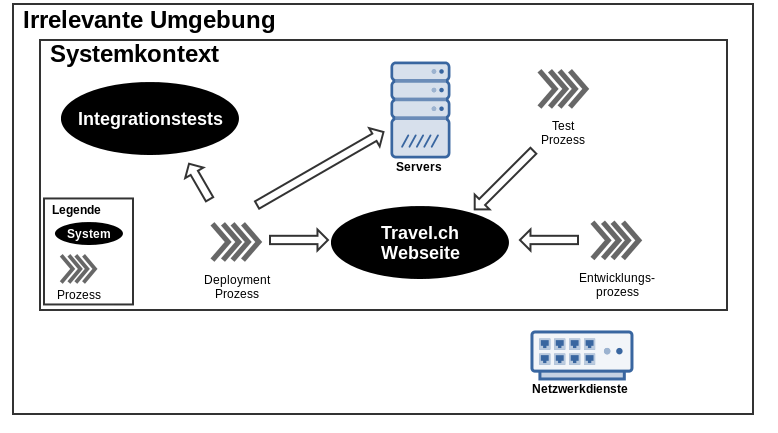
\includegraphics[width=0.8\textwidth]{images/Semesterarbeit Systemkontext.png}
	\caption{Systemkontext}
	\label{fig:analyse:systemkontext}
\end{figure}
Der Systemkontext besteht hauptsächlich aus den beiden Systemen \textit{Integrationstests} und \textit{travel.ch Webseite}. Die Integrationstests werden während diesem Projekt entwickelt und Testen die Webseite travel.ch.

Zusätzlich müssen die Tests in den \textit{Deployment Prozess} integriert werden, weshalb dieser auch zum Systemkontext gezählt werden muss. Weitere Informationen zu diesem Prozess sind im \cref{sec:umsetzung:infrastruktur} \nameref{sec:umsetzung:infrastruktur} und im \cref{sec:umsetzung:architektur:bootstrap:konfiguration} \nameref{sec:umsetzung:architektur:bootstrap:konfiguration} zu finden.

Der Test Prozess wird vor jedem Deployment der travel.ch Webseite durchgeführt. Die Integrationstests haben Einfluss darauf, da sie den diese Arbeit durch Automatisation erleichtern sollen (siehe \cref{sec:desc:targets} \nameref{sec:desc:targets}).

Während dem \textit{Entwicklungsprozess} für die travel.ch Webseite nach dem Projekt müssen die Funktionalitäten, welche im \cref{app:Funktionalitäten} \nameref{app:Funktionalitäten} aufgeführt sind, weiter gepflegt werden. Dadurch weiss eine Testperson, welche Funktionalitäten automatisch überprüft werden und nicht mehr manuell überprüft werden müssen.

Nicht Teil des Systemkontext sind betroffene Netzwerkdienste, welche für die Testdurchführung betroffen sind. Diese liegen ausserhalb des Einflussbereiches der Entwickler und werden innerhalb der Firma von einer anderen Abteilung gepflegt.

\section{Anforderungsdreieck}
Es gibt folgendes Anforderungsdreieck an die Testsuite:
\begin{figure}[H]
	\centering
	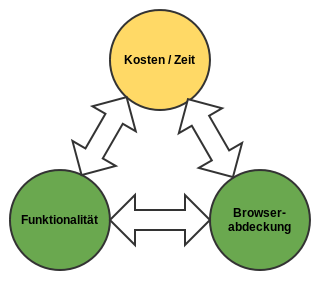
\includegraphics[width=0.6\textwidth]{images/triangle.png}
	\caption{Anforderungsdreieck}
	\label{fig:analyse:Anforderungsdreieck}
\end{figure}
Die Funktionalität und die Browserabdeckung sind funktionale Anforderungen. Bei den Kosten und der Zeit handelt es sich hingegen um nicht funktionale Anforderungen.

Je mehr Funktionalität abgedeckt wird, desto länger dauern die Tests. Und für jeden Browser müssen nochmals alle Tests durchgeführt werden. Deshalb stehen "`Kosten / Zeit"' im Widerspruch mit der Funktionalität und der Browserabdeckung.

Diese Anforderungen sind in den nächsten Abschnitten beschrieben.

\subsection{Funktionalität}
\label{sec:analyse:Funktionalität}
Die gesamte Funktionalität der Webseite, inklusive der Priorisierung, ist im \cref{app:Funktionalitäten} \nameref{app:Funktionalitäten} aufgelistet. Die Liste wurde im Wiki von der Hotelplan Management AG erstellt. Diese soll auch nach der Arbeit weiter gepflegt werden und wurde deshalb so aufgebaut, dass sie sehr übersichtlich ist und einfach bearbeitet und erweitert werden kann.

Vor dieser Arbeit gab es keine Dokumente, welche die Funktionalität der Webseite beschrieb. Deshalb musste die gesamte Funktionalität durch Analyse der bestehenden Seite rekonstruiert werden (reverse engineering).

Ziel ist es, die gesamte Funktionalität der Webseite zu testen.

\subsection{Browserabdeckung}
Im \cref{sec:Recherche:Zielgruppe} \nameref{sec:Recherche:Zielgruppe} sind die meist verwendeten Browser aufgelistet. Der Vorteil der Service-Anbieter ist, dass es sehr leicht ist eine Testsuite auf einem weiteren Webbrowser auszuführen. 

Wenn möglich sollten alle Browser aus der Recherche geprüft werden. Es ist jedoch zu eruieren wie lange die Tests brauchen, um durchzulaufen. Dann kann entschieden werden, im Betracht der Kosten, auf wie vielen Browsern die Testsuite durchgeführt wird. Diese Entscheidung wird mit dem Business der travelwindow AG getroffen, da sie den Kostenrahmen der Tests bestimmen.

\subsection{Kosten und Zeit}
Die Laufzeit der Test bestimmt die anfallenden kosten, da die Service-Anbieter pro Minute abrechnen, welche die Tests auf ihren Systemen laufen. Die Kosten, und demnach die Zeit, sollten so klein wie möglich gehalten werden. Je höher jedoch die Browserabdeckung und die getestete Funktionalität ist, desto länger dauern die Tests.

Je nachdem, wie lange die Tests benötigen, kann über die Anzahl der Browser, auf denen die Tests laufen gelassen werden sollen, die Kosten gesteuert werden.

\subsection{Kompromis}
\label{sec:analyse:testabdeckung}
Um ein Gleichgewicht zwischen Funktionalität, Browserabdeckung und "`Kosten \& Zeit"' zu waren wurde mit dem Business von travel.ch entschieden, dass alle Anforderungen im \cref{app:Funktionalitäten} \nameref{app:Funktionalitäten} mit einer Priorität von 8 oder höher zu testen sind. Zusätzlich wurde festgelegt, dass die beiden Browserversionen Safari 8.0 und Internet Explorer 11.0 getestet werden sollen.

Dadurch sollen die Testpersonen entlastet werden, da die wichtigsten Funktionalitäten getestet werden. Eine Abdeckung von 100\% ist anzustreben, jedoch innerhalb des Projekts nicht realistisch.

Falls sich nach dem Projekt die Tests als hilfreich herausstellen wird das Budget erhöht und die Browserabdeckung kann erweitert werden.

\section{Grenzwertanalyse}
\label{sec:analyse:grenzwertanalyse}
Dieser Abschnitt befasst sich mit der Grenzwertanalyse\footcite{Dynamisches_Software-Testverfahren__Wikipedia_2015-10-25} der Suchparameter. Diese soll alle zu testenden Parameter liefern, welche in den Suchmasken der travel.ch Webseite eingegeben werden können.

\subsection{Abflughafen}
Bei der CityTrip Engine gibt es folgende feste Anzahl an möglichen Abflughäfen.
\begin{itemize}
\item Zürich
\item Basel-Mülhausen
\item Genève-Cointrin
\item Bern-Belp
\item Lugano
\end{itemize}

Die Flug Engine gibt keine Abflughafen vor. Es kann von allen möglichen Abreiseorte gewählt werden.
Beim Buchen eines Hotels ist diese Auswahl hinfällig, da nur ein Reiseziel gewählt werden muss und kein Abflughafen.

\subsection{Passagierangaben}
Die Passagierangaben sind für die Engines CityTrip und Hotels die selben, jedoch für Flüge unterschiedlich, da keine Zimmerbelegung angegeben werden muss. Nachfolgend sind deshalb die möglichen Werte für CityTrip und Hotels zusammengefasst.\\
\\  
\noindent CityTrip und Hotels:
\begin{itemize}
\item Minimum Anzahl an Zimmer: 1
\item Maximum Anzahl an Zimmer: 3
\item Minimum Anzahl an erwachsenen Personen: 1
\item Maximum Anzahl an erwachsenen Personen: 6
\item Minimum Anzahl an Kinder: 0
\item Maximum Anzahl an Kinder: 4
\item Maximum Alter der Kinder: 18
\end{itemize}

\subsection{Datumsangaben}
Für jede Engine muss ein Start- und ein Enddatum ausgewählt werden. Diese werden über eine Kalenderauswahl eingegeben. Dabei gibt es pro Engine verschiedene Bereiche, aus denen die Daten ausgewählt werden können.\\
\\  
\noindent CityTrip:
\begin{itemize}
\item Frühstes Datum: Heute + 3 Tage
\item Letztes Datum: Heute + 1 Jahr - 1 Tag
\item Kürzeste Aufenthaltsdauer: 1 Tag
\end{itemize}
\vspace{0 mm}
Flug:
\begin{itemize}
\item Frühstes Datum: Heute + 3 Tage
\item Letztes Datum: Heute + 1 Jahr
\item Kürzeste Aufenthaltsdauer: 1 Tag
\end{itemize}
\vspace{0 mm}
Hotel:
\begin{itemize}
\item Frühstes Datum: Heute
\item Letztes Datum: Heute + 2 Jahre
\item Kürzeste Aufenthaltsdauer: 1 Tag
\end{itemize}

\subsection{Erweiterte Suche}
In der erweiterten Suche gibt es weitere Suchparameter, welche fakultativ für die Verfeinerung der Resultate angegeben werden können:

\subsubsection{Hotelklasse}
Die Hotelklasse kann bei CityTrip und Hotel gewählt werden. Von den folgenden Werten können einer oder mehrere selektiert werden:
\begin{itemize}
\item 0 Stern
\item 1 Stern
\item 2 Stern
\item 3 Stern
\item 4 Stern
\item 5 Stern
\end{itemize}

\subsubsection{Bewertungen}
Die Bewertungen können bei CityTrip und Hotel gewählt werden. Von den folgenden Werten kann einer selektiert werden:
\begin{itemize}
\item Alle
\item Hervorragend: 9+
\item Sehr Gut: 8+
\item Gut: 7+
\item Ansprechend: 6+
\item Ohne Bewertung
\end{itemize}

\subsubsection{Verpflegung}
Die Verpflegung kann bei CityTrip und Hotel gewählt werden. Von den folgenden Werten können einer oder mehrere selektiert werden:
\begin{itemize}
\item Ohne Mahlzeit
\item Frühstück
\item Halbpension
\item Vollpension
\item All-inclusive
\end{itemize}

\subsubsection{Flugoptionen}
Die Flugoptionen kann bei CityTrip und Flug gewählt werden. Von den folgenden Werten können einer oder mehrere selektiert werden:
\begin{itemize}
\item Direktflug
\item Mit Gepäck
\item Ohne Gepäck
\end{itemize}

\subsubsection{Verbindungsoptionen}
Die Verbindungsoptionen kann bei Flug gewählt werden. Von den folgenden Werten kann einer selektiert werden:
\begin{itemize}
\item Hin-/Rückflug
\item Andere Rückflugstrecke
\item Nur Hinflug
\end{itemize}

\subsubsection{Airline}
Die Airline kann bei Flug gewählt werden. Dabei handelt es sich um Airlines oder Allianzen\footcite{Airline_alliance}, welche auch mit einander nach belieben kombiniert werden können. Der Benutzer kann keine, eine oder mehrere Optionen selektieren. Die gesamte Liste der Airlines ist im \cref{app:airlines} \nameref{app:airlines} aufgeführt.